\section{Model 3: Performance Impact and Aging}
\label{sec:model3}

\hspace*{\parindent}In practice, prolonged usage induces battery aging, resulting in a reduction of effective capacity; the impact of this phenomenon on smartphone battery performance cannot be ignored. Specifically, lithium-ion batteries undergo performance degradation through two primary mechanisms: calendar aging and cycle aging \cite{Bloom2001, Wang2014, Barr2013}.


\subsection{Calendar Aging Model}
\label{subsec:calendar_aging}

\hspace*{\parindent}Calendar aging follows a square-root-of-time dependence:

\begin{equation}
    \frac{dSOH_{\text{cal}}}{dt} = -k_{\text{cal}}(T, SOC) = -A_{\text{cal}} \cdot \exp\left(-\frac{E_{a,\text{cal}}}{R_{\text{gas}} T}\right) \cdot f_{\text{SOC}}(SOC)
    \label{eq:calendar_aging}
\end{equation}

\textbf{SOC stress factor:}
\begin{equation}
    f_{\text{SOC}}(SOC) = \exp\bigl(\beta \cdot (SOC - 0.5)\bigr)
\end{equation}

\hspace*{\parindent}Where, $\beta$ represents the SOC stress exponent, a positive value (typically on the order of 10--30). Calendar aging stems from continuous internal chemical side reactions occurring while the battery is in an idle state, driven primarily by temperature and the state of charge (SOC). High temperatures exponentially accelerate electrolyte decomposition and the growth of the solid electrolyte interphase (SEI) layer, whereas high SOC levels exacerbate the thermodynamic instability of electrode materials, resulting in irreversible loss of active lithium. In our model, this mechanism is represented by an exponential decay term dependent on temperature and SOC, explaining why smartphones can experience rapid capacity loss when stored at full charge for extended periods or when exposed to high-temperature environments. Figure~\ref{fig:calendar_aging} illustrates the calendar aging behavior under various temperature and SOC conditions.

\begin{figure}[htbp]
    \centering
    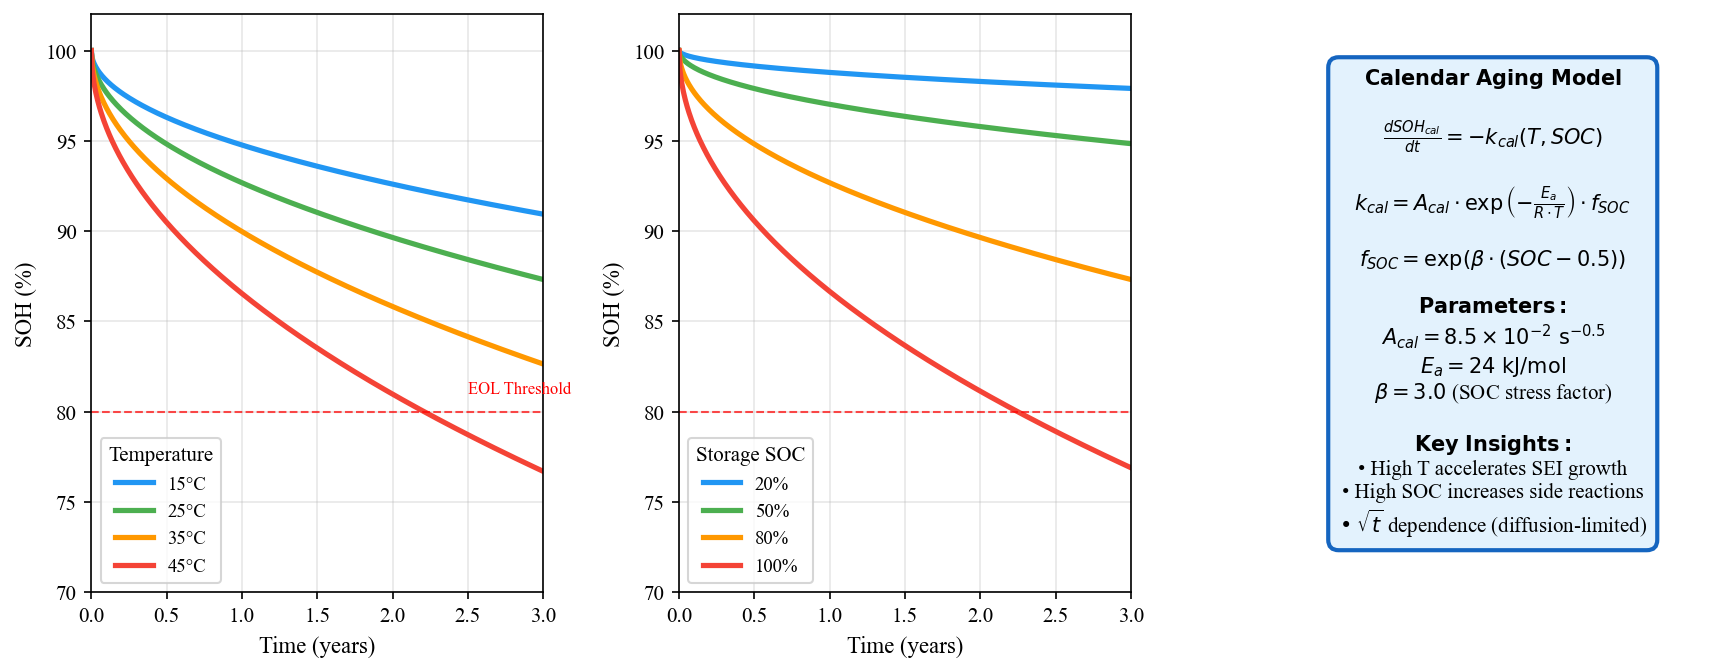
\includegraphics[width=0.85\textwidth]{fig7_calendar_aging.png}
    \caption{Calendar aging model results. (a) SOH degradation over time at different temperatures ($T$ = 15°C, 25°C, 35°C, 45°C) with SOC = 50\%. (b) SOH degradation at different SOC levels (20\%, 50\%, 80\%, 100\%) at $T$ = 25°C. Higher temperatures and higher SOC levels accelerate calendar aging.}
    \label{fig:calendar_aging}
\end{figure}

\begin{figure}[htbp]
    \centering
    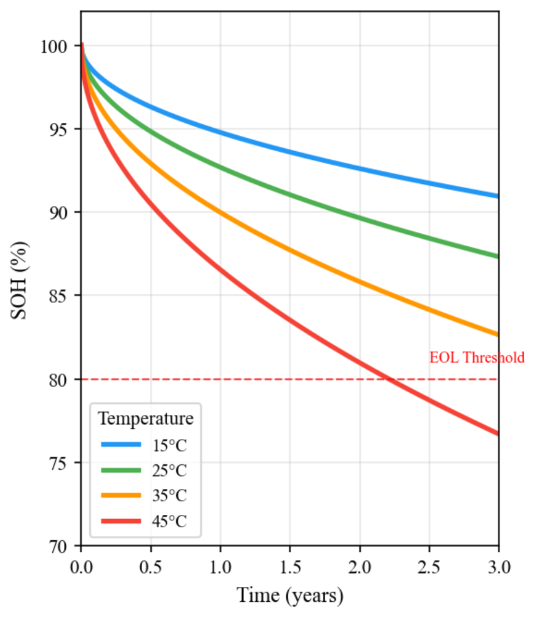
\includegraphics[width=0.75\textwidth]{figures/322F00FBCC307C716C0750AC0513D602.png}
    \caption{Effect of temperature on calendar aging: SOH degradation over 3 years at different ambient temperatures (15°C, 25°C, 35°C, 45°C). The red dashed line indicates the 80\% EOL threshold. Batteries stored at 45°C reach end-of-life approximately 2.3 years earlier than those at 15°C.}
    \label{fig:calendar_aging_temp}
\end{figure}

\begin{figure}[htbp]
    \centering
    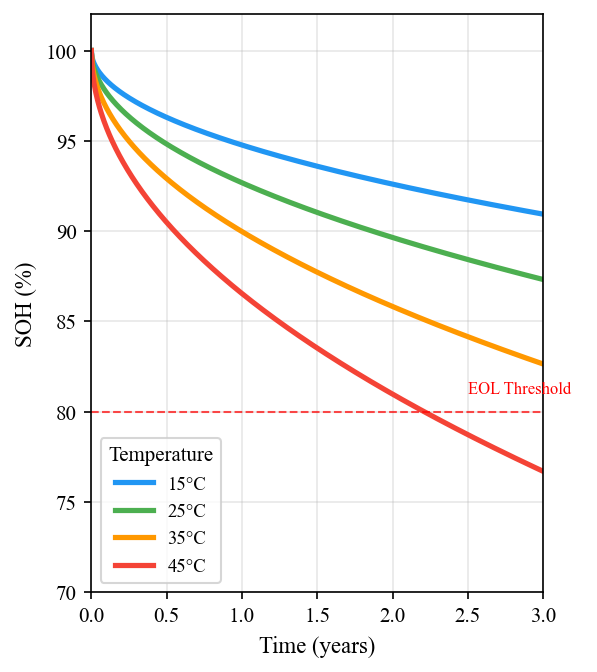
\includegraphics[width=0.75\textwidth]{figures/figure/D25663D19989A12F128F8E598BA1CCA8.png}
    \caption{Temperature-dependent calendar aging visualization showing SOH degradation over 3 years at temperatures of 15°C, 25°C, 35°C, and 45°C. The 80\% EOL threshold (dashed line) illustrates that higher storage temperatures dramatically accelerate capacity loss.}
    \label{fig:calendar_aging_temp_alt}
\end{figure}

\begin{figure}[htbp]
    \centering
    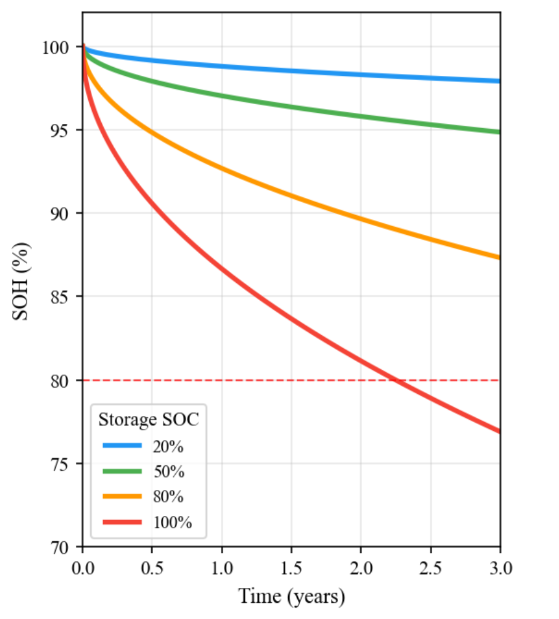
\includegraphics[width=0.75\textwidth]{figures/68404D8809850AAEDEB4075986A53E6F.png}
    \caption{Effect of storage SOC on calendar aging: SOH degradation over 3 years at different storage states (20\%, 50\%, 80\%, 100\% SOC). Storing batteries at full charge (100\% SOC) accelerates degradation significantly, crossing the 80\% EOL threshold around 2.4 years.}
    \label{fig:calendar_aging_soc}
\end{figure}

\begin{figure}[htbp]
    \centering
    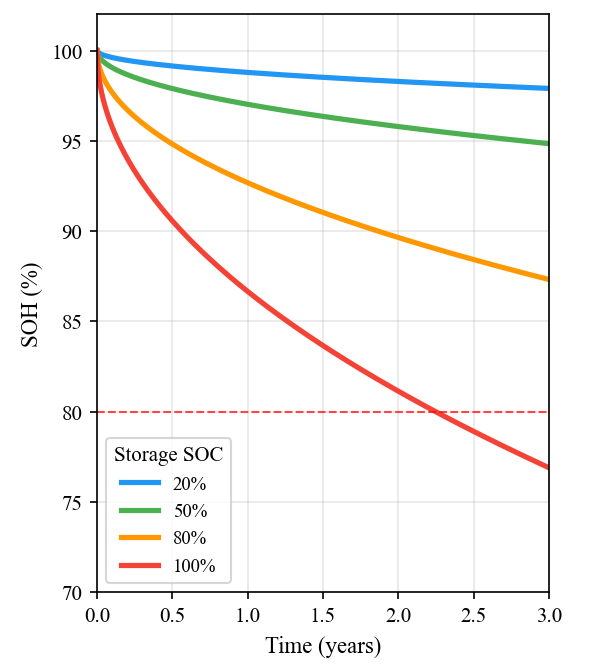
\includegraphics[width=0.75\textwidth]{figures/figure/FE73B8FCDA04CD1D811964A4634C532E.png}
    \caption{SOC-dependent calendar aging behavior showing SOH evolution at different storage charge levels (20\%, 50\%, 80\%, 100\% SOC). The exponential SOC stress factor causes batteries stored at high SOC to degrade significantly faster, with 100\% SOC storage crossing the 80\% threshold approximately 1.5 years earlier than 20\% SOC storage.}
    \label{fig:calendar_aging_soc_alt}
\end{figure}

\begin{figure}[htbp]
    \centering
    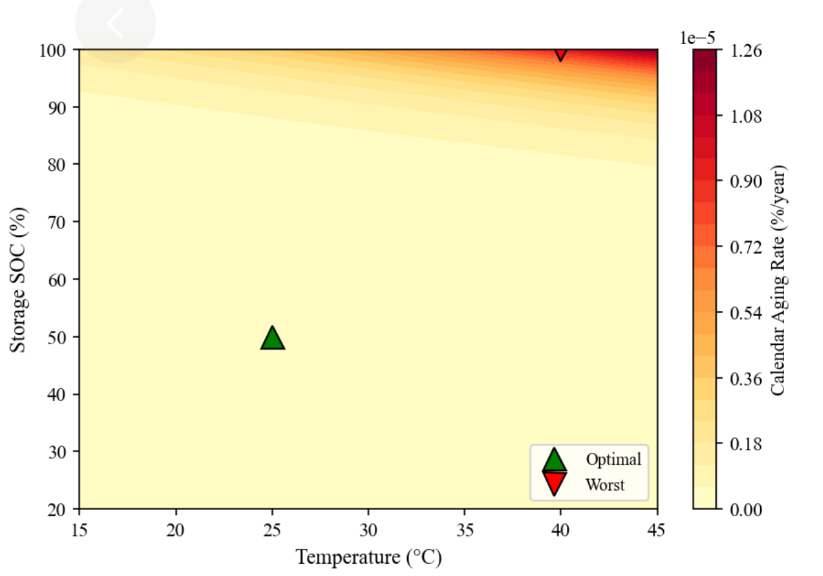
\includegraphics[width=0.7\textwidth]{figures/4B73C9E1BD96A2F7D75895EF46CCC960.png}
    \caption{Calendar aging rate heatmap as a function of temperature and storage SOC. The optimal storage condition (green marker) is at low temperature and moderate SOC, while the worst condition (red marker) is at high temperature and high SOC.}
    \label{fig:calendar_aging_heatmap}
\end{figure}

\begin{figure}[htbp]
    \centering
    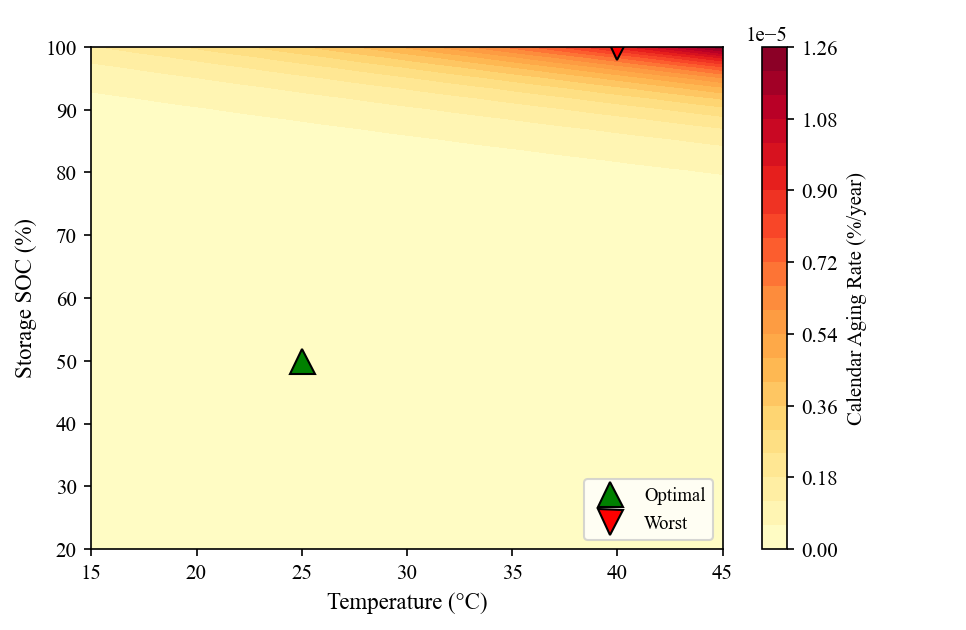
\includegraphics[width=0.7\textwidth]{figures/figure/0D13FA907D8ACDB51CF9B76BAC259460.png}
    \caption{Calendar aging rate contour plot showing degradation rate (\%/year) as a function of temperature (x-axis) and storage SOC (y-axis). Green triangle marks optimal conditions ($\sim$25°C, 50\% SOC), while red inverted triangle indicates worst conditions ($\sim$40°C, 100\% SOC). The color gradient visualizes the exponential relationship between aging rate and both temperature and SOC.}
    \label{fig:calendar_aging_contour}
\end{figure}

\begin{figure}[htbp]
    \centering
    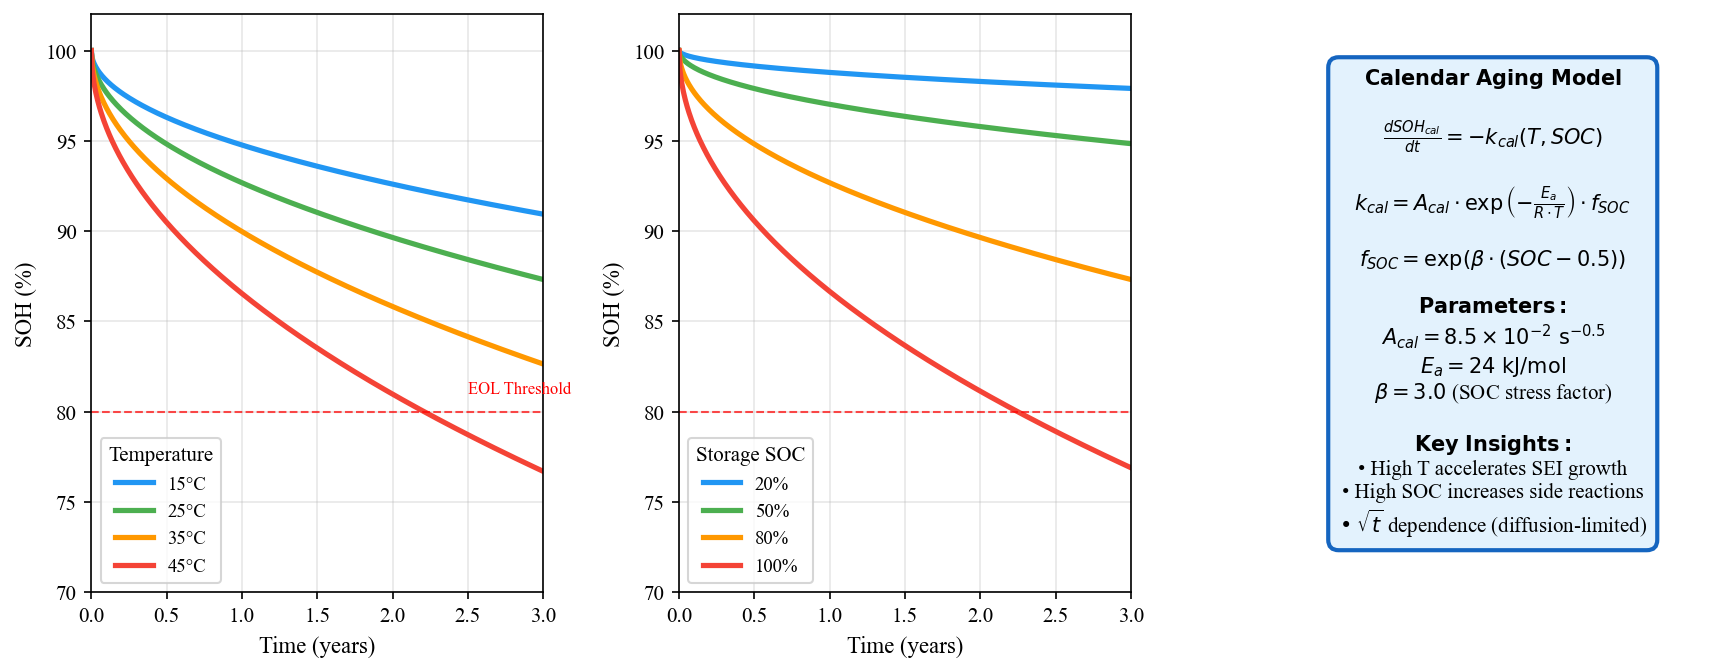
\includegraphics[width=\textwidth]{figures/figure/AEECB6B322D701D38D59A8D95A65E5D7.png}
    \caption{Comprehensive calendar aging analysis with model equations. Left panel: SOH degradation over time at different temperatures (15°C, 25°C, 35°C, 45°C). Middle panel: SOH degradation at different storage SOC levels (20\%, 50\%, 80\%, 100\%). Right panel: Calendar aging model formulation showing the Arrhenius temperature dependence and SOC stress factor, with key parameter values and insights.}
    \label{fig:calendar_aging_comprehensive}
\end{figure}

\subsection{Cycle Aging Model}
\label{subsec:cycle_aging}

Cycle aging depends on depth of discharge (DOD) and charge/discharge rate:

\begin{equation}
    \frac{dSOH_{\text{cyc}}}{dt} = -k_{\text{cyc}}(T) \cdot \text{DOD}^{\gamma} \cdot \left(\frac{I}{I_{\text{nom}}}\right)^{\alpha} \cdot |I|
    \label{eq:cycle_aging}
\end{equation}

where: $k_{\text{cyc}}(T)$ represents the aging rate constant, which is a function of temperature $T$.$\gamma \approx 2.0$ is the depth of discharge (DOD) exponent$\alpha \approx 0.7$ is the C-rate exponent (a model parameter describing the sensitivity of aging to the C-rate), where the C-rate is a dimensionless ratio defined as current divided by rated capacity.$I_{\text{nom}}$ represents the 1C discharge current.

Cycle aging arises from physicochemical fatigue during charge--discharge sequences, with the primary stress factors being the depth of discharge (DOD) and the current rate. Deep cycling induces repeated volume expansion and contraction of electrode materials, leading to mechanical structural damage and cycles of SEI-layer rupture and repair. Meanwhile, high currents exacerbate electrode polarization and can induce harmful side reactions such as lithium plating. Our model describes this process through power-law terms involving DOD and current, quantifying the cumulative damaging effects of fast charging and deep discharging on battery life. Figure~\ref{fig:cycle_aging} demonstrates the cycle aging behavior under various DOD and C-rate conditions.

\begin{figure}[htbp]
    \centering
    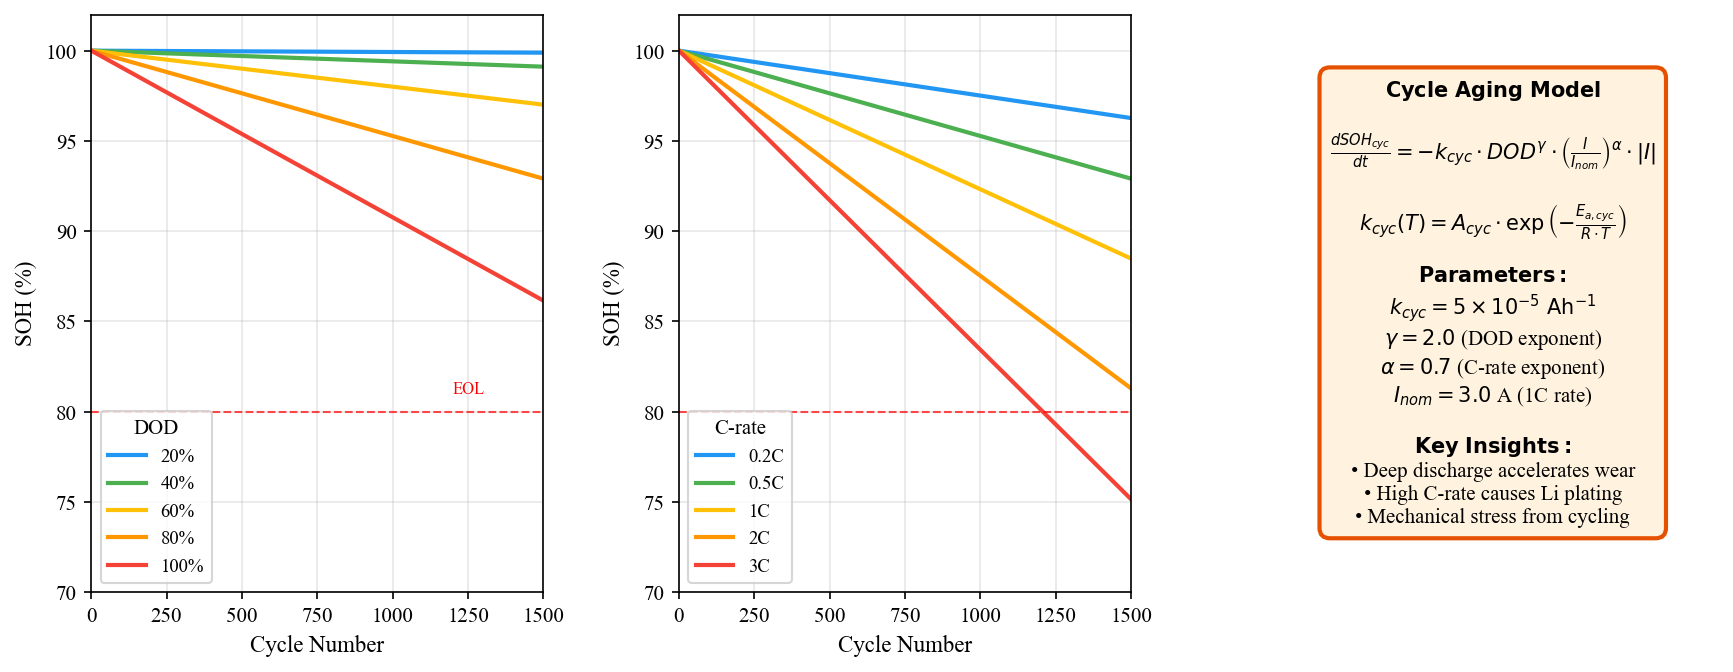
\includegraphics[width=0.85\textwidth]{fig8_cycle_aging.png}
    \caption{Cycle aging model results. (a) SOH degradation versus cycle number at different depths of discharge (DOD = 20\%, 50\%, 80\%, 100\%) with C-rate = 1C. (b) SOH degradation at different C-rates (0.5C, 1C, 2C, 3C) with DOD = 80\%. Deep cycling and high C-rates significantly accelerate cycle aging.}
    \label{fig:cycle_aging}
\end{figure}

\begin{figure}[htbp]
    \centering
    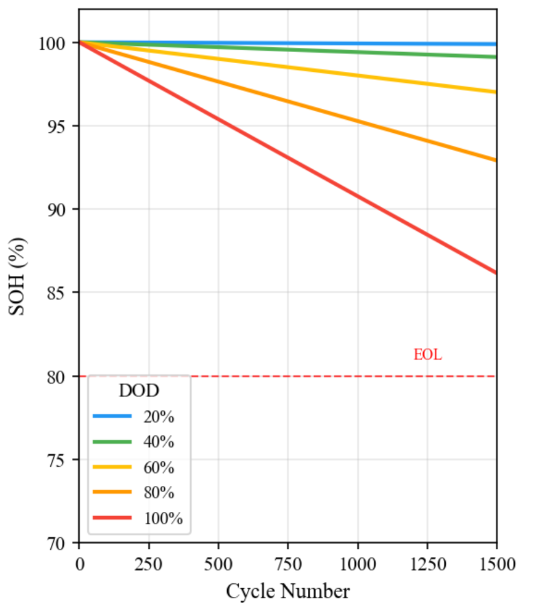
\includegraphics[width=0.75\textwidth]{figures/E714A144D33DAEA34987E2AF570B898A.png}
    \caption{Effect of depth of discharge (DOD) on cycle aging: SOH degradation over 1500 cycles at different DOD levels (20\%, 40\%, 60\%, 80\%, 100\%). Full depth discharges (100\% DOD) cause the most severe degradation, approaching the 80\% EOL threshold.}
    \label{fig:cycle_aging_dod}
\end{figure}

\begin{figure}[htbp]
    \centering
    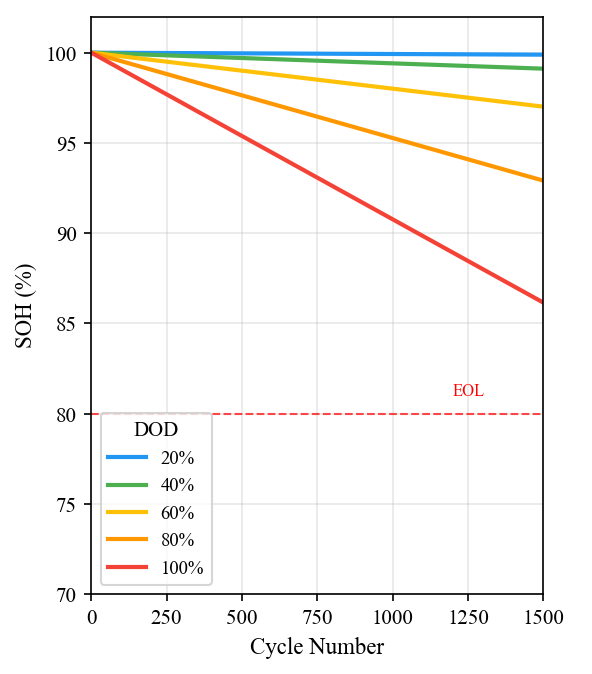
\includegraphics[width=0.75\textwidth]{figures/figure/796EB45EACC270DC63389E6D967DB351.png}
    \caption{DOD-dependent cycle aging analysis showing SOH degradation over 1500 cycles at different depths of discharge (20\%, 40\%, 60\%, 80\%, 100\%). The horizontal dashed line indicates the 80\% EOL threshold, demonstrating that 100\% DOD cycling approaches this limit while shallow cycling (20\% DOD) maintains high SOH.}
    \label{fig:cycle_aging_dod_alt}
\end{figure}

\begin{figure}[htbp]
    \centering
    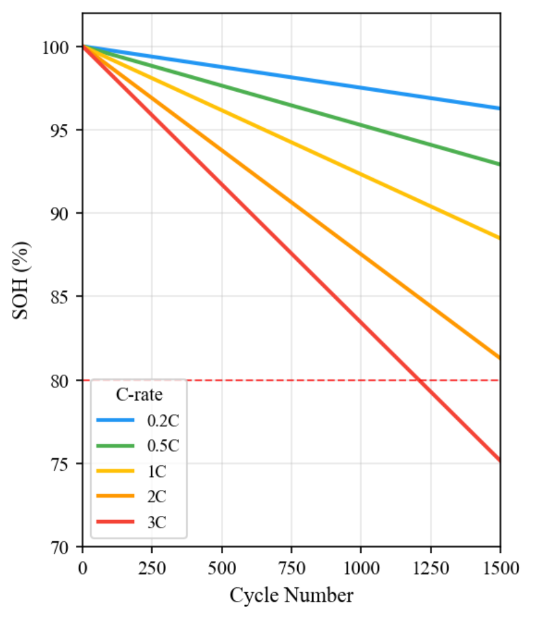
\includegraphics[width=0.75\textwidth]{figures/64E75C45C706D909BF9217CDBD0AAAEE.png}
    \caption{Effect of C-rate on cycle aging: SOH degradation over 1500 cycles at different charging/discharging rates (0.2C, 0.5C, 1C, 2C, 3C). Higher C-rates accelerate capacity fade, with 3C operation reaching approximately 75\% SOH at 1500 cycles.}
    \label{fig:cycle_aging_crate}
\end{figure}

\begin{figure}[htbp]
    \centering
    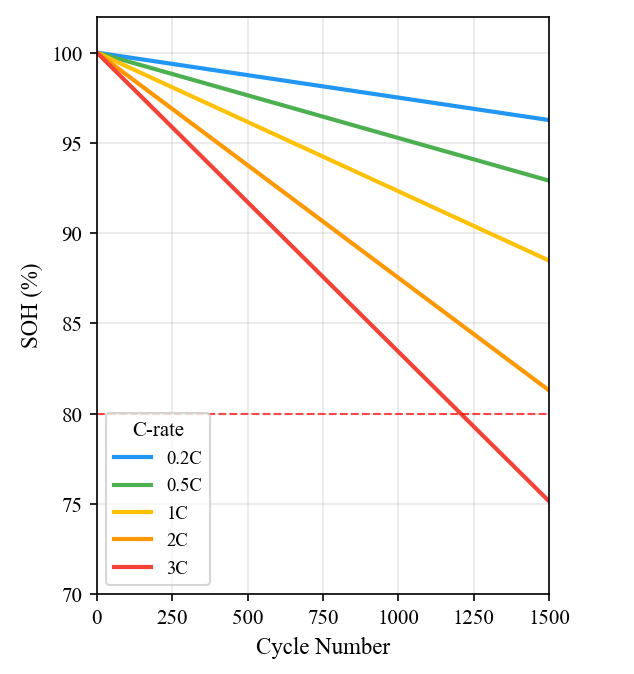
\includegraphics[width=0.75\textwidth]{figures/figure/57804EFD4BFF0A13BF83FD3CB652ED8C.png}
    \caption{C-rate dependent cycle aging behavior showing SOH evolution at different charge/discharge rates (0.2C, 0.5C, 1C, 2C, 3C). The 80\% EOL threshold (dashed line) demonstrates that aggressive fast charging (3C) significantly reduces battery lifespan compared to standard charging rates.}
    \label{fig:cycle_aging_crate_alt}
\end{figure}

\subsection{Combined Aging Model}
\label{subsec:combined_aging}

\begin{equation}
    \boxed{\frac{dSOH}{dt} = -\dot{SOH}_{\text{cal}}(T, SOC) - \dot{SOH}_{\text{cyc}}(I, T, SOC)}
    \label{eq:total_aging}
\end{equation}

Based on the integrated aging model, it is evident that smartphone battery aging is the result of the combined action of calendar aging and cycle aging.Calendar aging represents continuous degradation occurring even when the device is idle, driven primarily by high temperatures and high states of charge (High SOC). Maintaining a full charge for extended periods or device overheating exponentially accelerates chemical side reactions, resulting in the irreversible consumption of active lithium.Cycle aging occurs during every charge-discharge cycle; deep discharges (high-intensity usage at low battery levels) and high currents from fast charging exacerbate the structural fatigue of electrode materials and the proliferation of the SEI layer.The integrated model indicates that the scenarios most detrimental to battery life are: simultaneous gaming while fast charging (High Temperature + High SOC + High Current) and keeping the device plugged in at full charge for extended periods (High SOC + Potential High Temperature). Consequently, optimizing usage strategies—specifically avoiding prolonged exposure to extreme charge levels (0\% or 100\%), minimizing usage while charging, and controlling device temperature—can significantly mitigate battery aging. Figure~\ref{fig:comprehensive_aging} presents a comprehensive comparison of aging under different usage scenarios.

\begin{figure}[htbp]
    \centering
    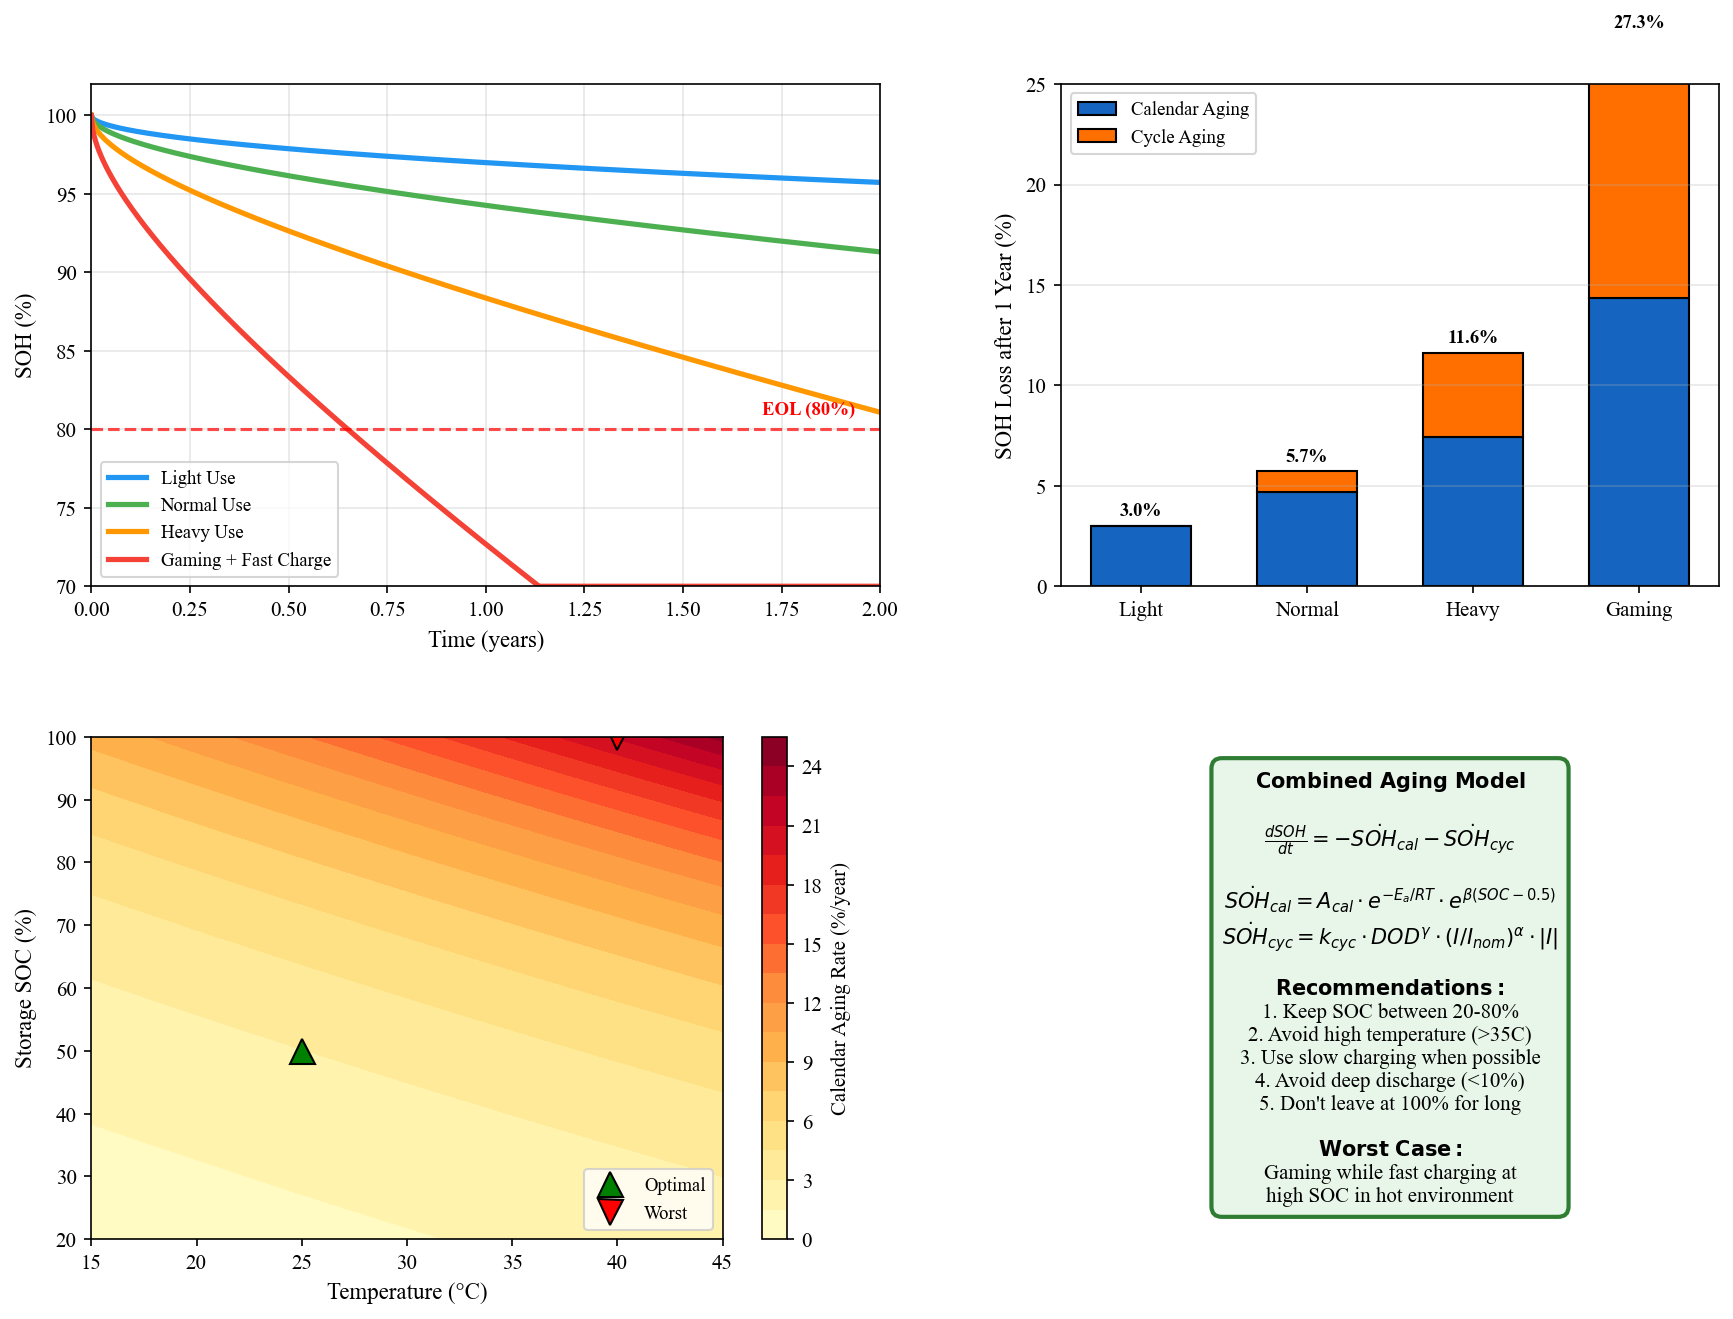
\includegraphics[width=\textwidth]{fig9_comprehensive_aging.png}
    \caption{Comprehensive aging model analysis. (a) Combined SOH degradation trajectories for different usage scenarios over 3 years: Light Use (20--80\% SOC, 0.5C, 25°C), Normal Use (10--90\% SOC, 1C, 30°C), and Gaming + Fast Charge (0--100\% SOC, 2C, 40°C). (b) Stacked bar chart showing calendar vs.\ cycle aging contributions for each scenario. (c) Heatmap of time to reach 80\% EOL threshold as a function of average C-rate and temperature, demonstrating the strong dependence on both factors.}
    \label{fig:comprehensive_aging}
\end{figure}

\begin{figure}[htbp]
    \centering
    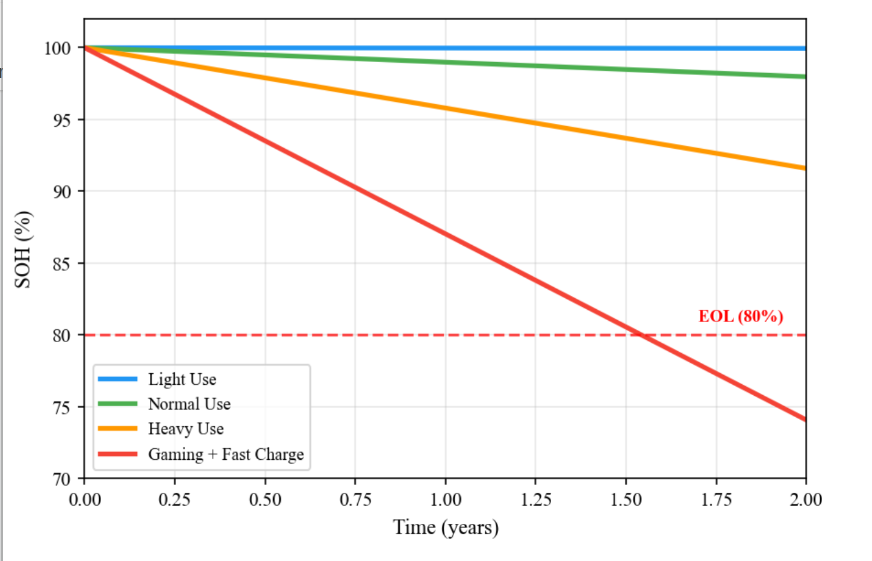
\includegraphics[width=0.8\textwidth]{figures/3A12E2E1BB085F3455F77B49F45853AB.png}
    \caption{Long-term SOH projection for different usage profiles over 2 years. Light Use maintains $>$98\% SOH, while Gaming + Fast Charge drops below the 80\% EOL threshold around 1.5 years. The stark contrast highlights the importance of usage habits on battery longevity.}
    \label{fig:soh_projection}
\end{figure}

\begin{figure}[htbp]
    \centering
    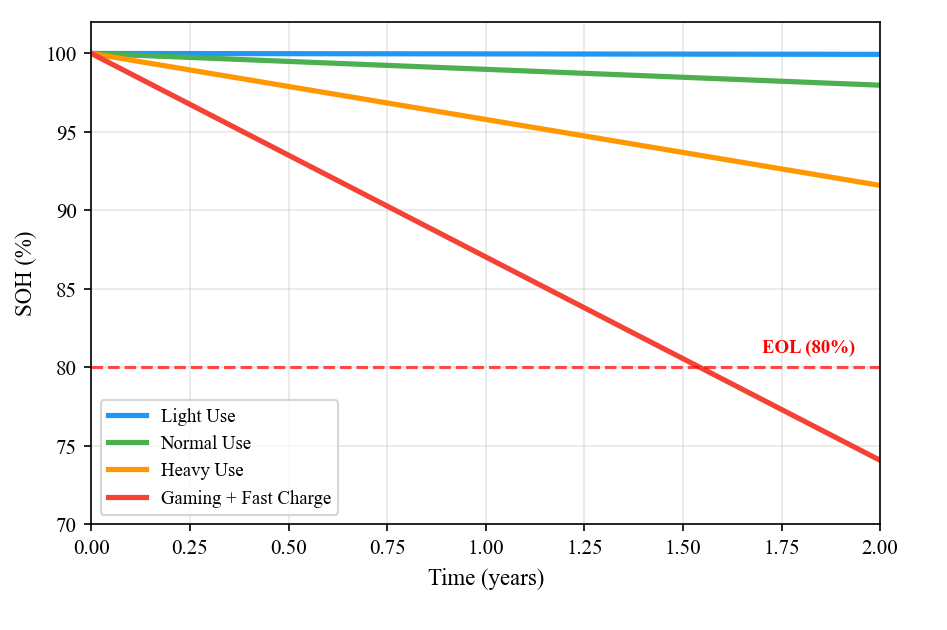
\includegraphics[width=0.8\textwidth]{figures/figure/82FE5C28F577DF0A26BF41518A1A7F4A.png}
    \caption{Alternative long-term SOH projection visualization showing battery health evolution over 2 years for Light Use, Normal Use, Heavy Use, and Gaming + Fast Charge profiles. The EOL threshold (80\% SOH) clearly differentiates sustainable usage patterns from aggressive ones that rapidly degrade battery capacity.}
    \label{fig:soh_projection_alt}
\end{figure}

\begin{figure}[htbp]
    \centering
    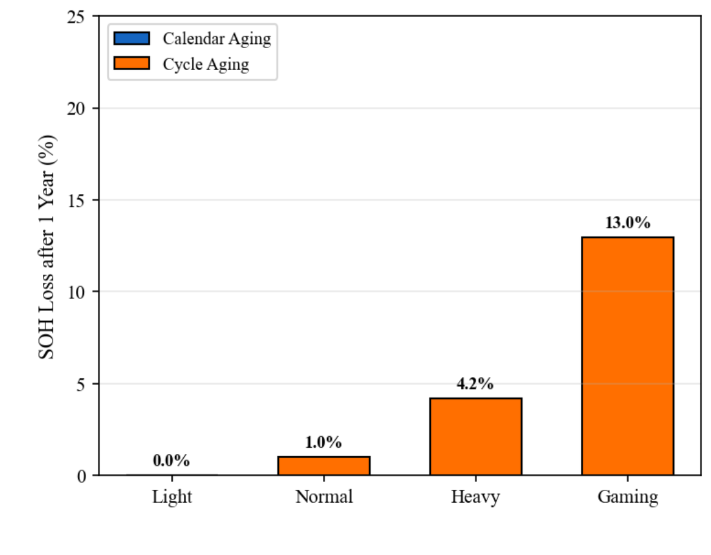
\includegraphics[width=0.75\textwidth]{figures/AB9BE22B377F3DC74DBA21DAB9492FBE.png}
    \caption{Comparison of SOH loss after 1 year across different usage types. Gaming users experience 13.0\% capacity loss compared to only 1.0\% for normal users, with cycle aging being the dominant contributor.}
    \label{fig:soh_loss_comparison}
\end{figure}

\begin{figure}[htbp]
    \centering
    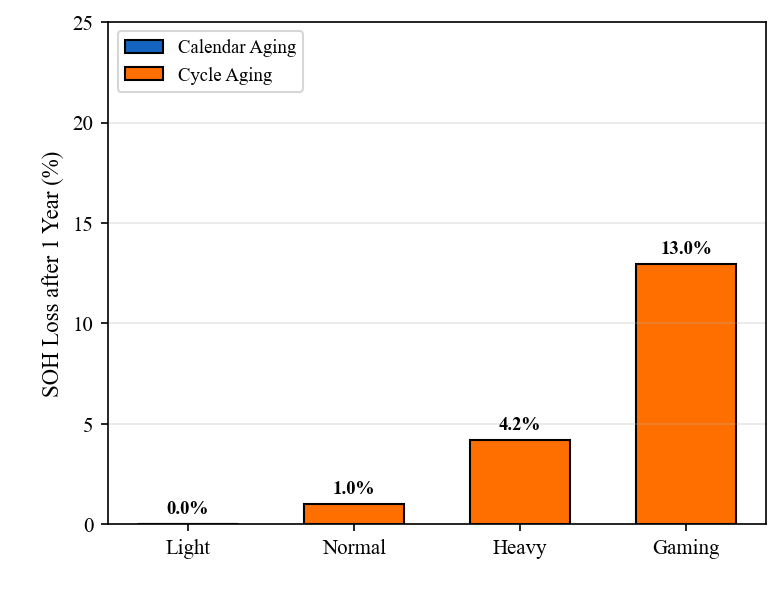
\includegraphics[width=0.75\textwidth]{figures/figure/576AC1221EE7B3BDCC9613AF3B955C02.png}
    \caption{Stacked bar chart showing SOH loss (\%) after 1 year by usage intensity. The orange bars represent cycle aging contribution, which dominates for heavy users. Light users experience negligible loss (0.0\%), Normal users 1.0\%, Heavy users 4.2\%, and Gaming users 13.0\%, demonstrating the exponential relationship between usage intensity and battery degradation.}
    \label{fig:soh_loss_stacked}
\end{figure}